% To je predloga za poročila o domačih nalogah pri predmetih, katerih
% nosilec je Blaž Zupan. Seveda lahko tudi dodaš kakšen nov, zanimiv
% in uporaben element, ki ga v tej predlogi (še) ni. Več o LaTeX-u izveš na
% spletu, na primer na http://tobi.oetiker.ch/lshort/lshort.pdf.
%
% To predlogo lahko spremeniš v PDF dokument s pomočjo programa
% pdflatex, ki je del standardne instalacije LaTeX programov.

\documentclass[a4paper,11pt]{article}
\usepackage{a4wide}
\usepackage{fullpage}
\usepackage[utf8x]{inputenc}
\usepackage[slovene]{babel}
\selectlanguage{slovene}
\usepackage[toc,page]{appendix}
\usepackage[pdftex]{graphicx} % za slike
\usepackage{setspace}
\usepackage{color}
\definecolor{light-gray}{gray}{0.95}
\usepackage{listings} % za vključevanje kode
\usepackage{hyperref}
\usepackage{float}
\usepackage{verbatim}
\renewcommand{\baselinestretch}{1.2} % za boljšo berljivost večji razmak
\renewcommand{\appendixpagename}{Priloge}

\lstset{ % nastavitve za izpis kode, sem lahko tudi kaj dodaš/spremeniš
language=Python,
basicstyle=\footnotesize,
basicstyle=\ttfamily\footnotesize\setstretch{1},
backgroundcolor=\color{light-gray},
}

\title{Tretja domača naloga}
\author{Anže Pečar (63060257)}
\date{\today}

\begin{document}

\maketitle

\section{Uvod}

Cilj domače naloge je bil oddati napovedi na tekmovalni stržnik in se seznaniti z ocenjevanjem točnosti in napovednimi modeli.

\section{Metode}
\subsection{Ocenjevanje točnosti}
Točnost svojih algoritmov sem ocenjeval s pomočjo F-ocene in $k$-stranskega prečnega preverjanja. F-ocena je definirana kot:
\[F = 2 * {Precision*Recall\over{Precision + Recall}},\]
kjer sta precision in recall:
\[ Precision = {\mid TrueTopics  \cap  PredictedTopics \mid \over{\mid PredictedTopics \mid}}, \]
\[ Recall = {\mid TrueTopics  \cap  PredictedTopics \mid \over{\mid TrueTopics \mid}}. \]
Za $k$-kratno prečno preverjanje sem implementiral lastno funkcijo, ki mi je vračala naključno razporejene indekse originalnih podatkov. S pomočjo tako pridobljenih indeksov sem učno množico $k$-krat razdelil na $k$ enakih delov.  Iz $k - 1$ delov sem zgradil svoj model, ki sem ga nato preizkusil na zadnjem delu. Končna F-ocena je povprečje vseh tako dobljenih F-ocen. Parameter $k$ je bil pri algoritmu 1R nastavljen na $5$, in je dokaj točno uspel napovedati tudi končno F-oceno, kot je tudi razvidno iz Tabele \ref{tabela}. Pri testiranju naključnih dreves pa sem naletel na problem s časovno kompleksnostjo. Generiranje modela 500tih dreves je trajalo kar dolgo:
\begin{verbatim}
real	889m59.265s
user	883m40.190s
sys	3m9.084s
\end{verbatim}
Zato sem prečno preverjanje poganjal s parametrom $k = 2$ in na modelu sestavljenim iz 10tih dreves. Posledica te odločitve so precej slabše F-ocene v Tabeli \ref{tabela}, kot pa tiste, ki sem jih dobil na strežniku. Kljub pomanjkljivostim pa so se te približne ocene izkazale kot dovolj dobre za nastavljanje parametrov algoritma (prag, normaliziran prag in dinamični prag), saj sem vsakič, ko sem uspel izboljšati lokalno F-oceno, dobil tudi boljšo F-oceno na strežniku. 
\subsection{Napovedni modeli}
\begin{itemize}
\item[1R] V knjigi \cite{mining} sem naletel na preprost algoritem imenovan 1R, ki sem ga nekoliko predelanega uporabil v domači nalogi. Algoritem deluje tako, da za vsak atribut prešteje razrede, ki jih določa. Za vsak atribut tako dobimo seznam razredov, ki jih je določil v učnih podatkih. Pri napovedovanju, združimo napovedane razrede vseh neničelnih atributov in izpišemo vse, ki imajo število ponovitev večje od določenega praga.
\item[1RS] Algoritem je zelo podoben algoritmu 1R, samo da namesto preprostega preštevanja razredov, seštevamo vrednosti atributov v danem primeru. Tako namesto števila razredov, dobimo seštevek vrednosti atributov. To nam izboljša napovedovanje za približno 7\%.
\item[RF] Naključne gozdove sem generiral za 10, 50, 250 in 500 dreves. Razlika med rezultatom z 250 drevesi in 500 so minimalne, v določenih primerih celo v prid 250 drevesi. Je pa zato toliko večja razlika med 250/500 drevesi in 50/10. V prvem tednu sem za izbiro napovedanih razredov uporabil samo pragovno vrednost (0.20 se je najbolje obnesla), v drugem tednu pa sem eksperimentiral z različnimi funkcijami.
\item[RFN] Prva taka funkcija je bila normalizacija dobljenih verjetnosti. Za posamezen testni primer sem verjetnosti vseh napovedanih razredov delil z najbolj verjetnim razredom in tako dobil normalizirane verjetnosti za posamezen primer. S pomočjo prečnega preverjanja sem nastavil normaliziran prag in izboljšal svoj rezultat za približno 2\%.
\item[RFDP] Verjetnosti razredov se med posameznimi primeri lahko kar precej razlikujejo. Statični oziroma normalizirani prag tega ne upošteva. Dinamični prag (DP) dobimo tako, da za osnovo vzamemo verjetnost najbolj verjetnega razreda in dovolimo določeno odstopanje od te verjetnosti po formuli 
\begin{verbatim}
x['predicted'] > sortedX[0]['predicted']*THRESH # sortedX[0] je najbolj 
                                                # verjeten razred.
\end{verbatim} 
\end{itemize}
\section{Rezultati}
Moje ime v tekmovalnem sistemu: Anže Pečar.
\subsection{Rezultati oddaj}
\begin{table}[H]
\caption{Oddaje}
\begin{tabular}{ c | c | c | c | c | p{6cm} }
  & Ime metode & Oddaja & ocena F &  F & Komentar\\
  \hline \hline
  * & 1R & 07.03. 13:31:56 & 0.33735 & 0.33878 & 1R s štetjem atributov \\ \hline
  * & 1RS &09.03. 09:18:21 & 0.36952 & 0.36384 & 1R s seštevamjem vrednosti atributov \\\hline
  * & RF &10.03. 09:44:08 & 0.38073 & 0.40977 & 250 dreves, prag 0.20, max 6 napovedanih razredov \\ \hline
  * & RF &11.03. 08:09:49 & 0.37891 & 0.40387 & 500 dreves, prag 0.20, max 6 napovedanih razredov \\ \hline
  & RFN &17.03. 16:02:10 & 0.38635 & 0.41439 & 500 dreves, normaliziran prag 0.5 \\ 
\hline
  & RFN &17.03. 23:29:35 & 0.38235 & 0.40337 & 500 dreves, normaliziran prag 0.1921 \\ \hline

  & RFDP &18.03. 12:53:21 & 0.39655 & 0.43659 & 500 dreves, dinamični prag 0.221 \\ 


 
 
 \end{tabular}
 \label{tabela}
\end{table}
V Tabeli \ref{tabela} je nekaj bolj zanimivih oddaj. Kot sem omenil že v poglavju o metodah, so lokalne napovedi ocene F pri naključnih drevesih precej slabše od tistih na strežniku zato, ker sem zaradi časovne kompleksnosti moral uporabiti slabši model za računanje. Zanimivo je tudi, da se je pod določenimi pogoji model z 250 drevesi obnesel bolje kot model s 500, vendar je bila to bolj izjema kot pravilo.
%\begin{figure}[H]
%\begin{center}
%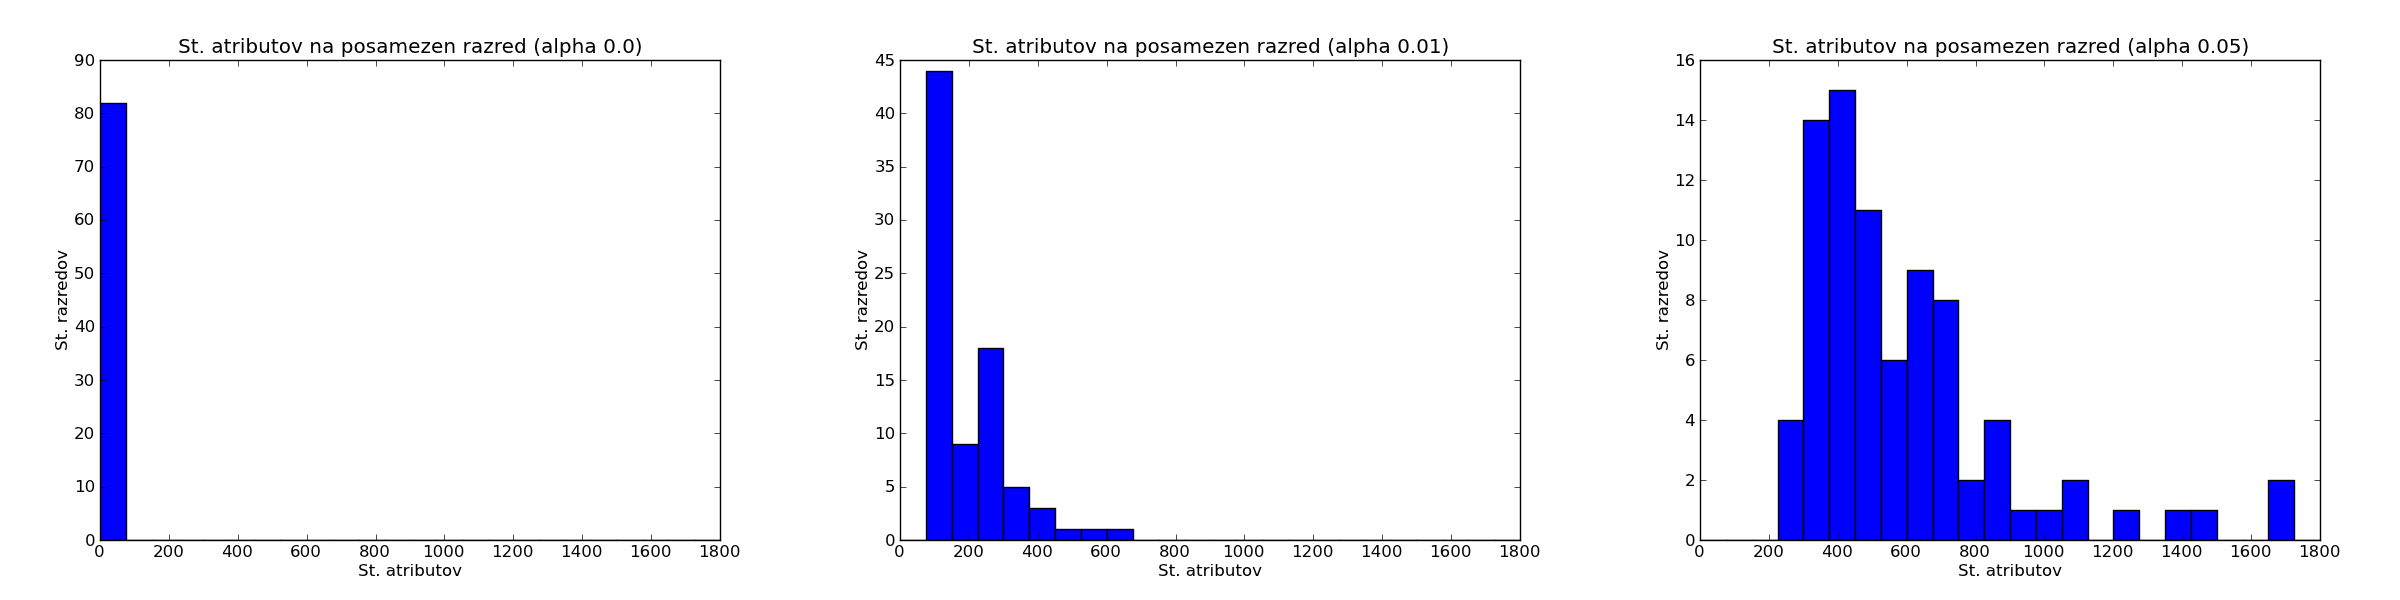
\includegraphics[scale=0.2]{skupno100.png}
%\caption{Rezultati 100 permutacij za različne vrednosti Alpha}
%\label{skupno100}
%\end{center}
%\end{figure}

\section{Izjava o izdelavi domače naloge}
Domačo nalogo in pripadajoče programe sem izdelal sam.


\begin{thebibliography}{9}

\bibitem{mining}
   Ian H. Witten \& Eibe Frank,
   \emph{Data Mining Practical Machine Learning Tools and Techniques, Second Edition}
   Morgan Kaufmann Publishers,  
   2005.

\end{thebibliography}

\end{document}
